%%%%%%%%%%%%%%%%%%%%%%%%%%%%%%%%%%%%%%%%%%%%%%%%%%%%%%%%%%%%%%%%%%%%%%%%%%%%%%%%%%%%%%%%%%%%%%%%%%
%%  Header of summary in Lithuanian, that used to set parameters of chapter counters, to set language and other parameters

%Change default parameters for Lithuanian language
\setcounter{section}{0}   %šita automatiškai atnaujina \appendix komanda
\renewcommand*{\thesection}{S.\arabic{section}}
\renewcommand{\thechapter}{S}
\renewcommand{\thefigure}{S.\arabic{figure}}   %raidė S įhardcodinta. Galima švelniau pvz su komanda \thechapter
\setcounter{figure}{0}
\renewcommand{\theequation}{S.\arabic{equation}}
\setcounter{equation}{0}
\renewcommand{\thetable}{S.\arabic{table}}
\setcounter{table}{0}
%jeigu yra dar ko nors, pvz algoritmu, teor ir pan, irgi reikia atnaujinti
\captionsetup[figure]{labelsep=space} %Lietuviškoje santraukoje nededame gale taško

\lithuanian   %nustatome lietuviu kalba
\sisetup{output-decimal-marker = {,}}  %lietuviski kableliai ir pan
\sisetup{exponent-product=\ensuremath{\cdot}}


\phantomsection
\chapter*{Summary in Lithuanian / Summary in English}
\label{cha:summary_lt}
\addcontentsline{toc}{chapter}{\MakeUppercase{Summary in Lithuanian - Summary in English}}

% NOTES to the author
% For chapter naming, please use APA style https://titlecapitalize.com/title-case-styles/
    % APA, or American Psychological Style, is one of the most commonly used title case styles in academia. It’s mainly used for research papers in social and behavioral sciences. 
    
    % Its title case rules are also easy enough to remember and follow. Capitalize all major words (nouns, pronouns, verbs, adjectives) in your title, as well as prepositions and conjunction with four or more letters. If your title includes a hyphenated word, capitalize both the initial letters before and after the hyphen. Lastly, the first word after a colon or dash is also capitalized when you’re following the APA style of capitalization for your title or headings.

\chapter*{Introduction / Įvadas}
\label{cha:intro_lt}
\addcontentsline{toc}{chapter}{\MakeUppercase{Introduction / Įvadas}} 

The dissertation must be an original scientific work that substantiates the research problem, defines the \textbf{relevance and purpose of the research work, formulates the goal and objectives of the thesis, indicates the novelty of the scientific work, presents defending statements of the thesis}, reviews the research conducted on the topic of the dissertation in the world (abroad and in Lithuania) and their results, presents the applied research methodology (methods), research results discussed, their reliability and relationship with the data of other researchers, conclusions formulated and other important aspects, in the dissertation's opinion.


\textbf{In Lithuanian}. Disertacija turi būti originalus mokslinis darbas, kuriame pagrindžiama \textbf{tiriamoji problema, apibrėžtas darbo aktualumas, tikslas, suformuluoti sprendžiami uždaviniai, nurodytas mokslinio darbo naujumas, ginami disertacijos teiginiai}, apžvelgti disertacijos tema pasaulyje (užsienyje ir Lietuvoje) atlikti tyrimai ir jų rezultatai, pristatyti taikyta tyrimų metodika (metodai), aptarti tyrimų rezultatai, pagrįstas jų patikimumas ir santykis su kitų tyrėjų duomenimis, suformuluotos išvados ir kiti, disertanto nuomone, svarbūs aspektai.


\phantomsection % Removes warning from hyperref package
\section*{Research Area / Tyrimų sritis}
\addcontentsline{toc}{section}{Research Area / Tyrimų sritis} 

In this section, we recommend briefly introducing the readers to the field of research, which is directly related to the research problem and the aim of the dissertation. Present the current situation in this research area, name the important and relevant research conducted in this area, and present their results. You can attach the research problem section to this section.

\textbf{In Lithuanian}.
Šiame skyrelyje rekomenduojame trumpai skaitytojus supažindinti su tyrimų sritimi, kuri tiesiogiai siejasi su su disertacijos problema ir tikslu. Pristatykite kokia yra dabar situacija šioje srityje, įvardinkite svarbius ir aktualius šioje srityje vykdomus tyrimus ir prisatykite jų rezultatus. Prie šio skyrelio galite prijunti tyrimo problemos skyrelį.

\section*{Research Problem / Tyrimo problema}
\addcontentsline{toc}{section}{Research Problem / Tyrimo problema} 

Definition. A perceived gap between the existing state and a desired state, or a deviation from a norm, standard, or status quo (Bussiness Dictionary\footnote{https://www.bussinessdictionary.com/definition/problem}).

Also:
\begin{itemize}
    \item A problem is a statement, in mathematics or physics, that indicates the need to do something.
    \item The problem is a complex unsolved question. 
    \item A scientific problem can be solved using the steps of the scientific method (e.g. experiments).
\end{itemize}
Before formulating a scientific problem, it is recommended to define the research object and formulate the problem using its concepts.


\textbf{In Lithuanian}. Apibrėžimas. \textbf{Problema} – tai tarpas tarp esamos būsenos ir siekiamos būsenos, arba nukrypimas nuo normos, standarto ar status quo.
Taip pat:
\begin{itemize}
    \item Problema – teiginys, matematikoje ar fizikoje, nurodantis poreikį kažką padaryti.
    \item Problema – sudėtingas neišspręstas klausimas. 
    \item Mokslinė problema – tai klausimas, kuris gali būti atsakytas naudojant mokslinius metodus (pvz., atliekant eksperimentus).
\end{itemize}
Prieš formuojant mokslinę promblemą rekomenduojama apsibrėžti tyrimo objektą ir naudojantis jo sąvokomis suformuluoti problemą.


\section*{Actuality / Darbo aktualumas}
\addcontentsline{toc}{section}{Actuality / Darbo aktualumas} 

The actuality of the research topic is the degree of its importance at the given moment and in this situation for solving these problems, a question or a problem\footnote{\url{https://en.ppt-online.org/424459}}.

In order to show the actuality of the research, you need:
\begin{itemize}
    \item to formulate the research problem
    \item to indicate contradictions found in science or practice that define the research problem
    \item to describe the current situation of the problem with a solution to the problem (is anyone still solving it?)
    \item to describe the importance of research work to society
    \item to generalize and to summarize the best results.
\end{itemize}

\textbf{In Lithuanian}.
Tyrimo temos aktualumas yra sprendžiamos problemos ar klausymo svarbos laipsnis šiuo momentu ir šiuoje situacijoje sprendžiant tyrimo sirties problemas.
Kad parodyti darbo aktualumą reikia:
\begin{itemize}
    \item suformuluoti tyrimo problemą,
    \item nurodyti prieštaravimus kurie aptinkami moksle arba praktikoje, kurie apibrėžia tyrimo problemą, 
    \item apibūdinti esamą problemos situaciją su problemos sprendimu (ar ją kas nors vis dar sprendžia?),
    \item darbo reikšmingumą visuomenei,
    \item apibendrinti geriausius rezultatus.
\end{itemize}


\section*{Research Object / Tyrimo objektas}
\addcontentsline{toc}{section}{Research Object / Tyrimo objektas} 

\textbf{Research object} or research subject is a thing (e.g. algorithm, person, data type) that is used in your research. The research object connects different research contexts: data, analysis tools, hypotheses, experiments, defending statements, and general conclusions. We recommend identifying from 3 to 5 main research concepts and formulating a coherent sentence from them as a research object.
These concepts should also be used in the thesis title and objective. You can read more about how to identify the object of your research on  \url{http://edutechwiki.unige.ch/en/Methodology_tutorial_-_finding_a_research_subject}.

\textbf{In Lithuanian}. \textbf{Tyrimo objektas} (angl. research object, research subject) – daiktas (pvz. algoritmas, asmuo, duomenų tipas), kuris naudojamas detaliame tyrime. Tyrimo objektas susieja skirtingus tyrimo kontekstus: duomenis, analizės įrankius, hipotezes, eksperimentus, ginamuosius teiginius ir išvadas. Rekomenduojame identifikuoti nuo 3 iki 5 pagrindinių tyrimo konceptų ir iš jų suformuluoti nuoseklų sakinį.
Šie konceptai taip pat turėtų būti panaudoti disertacijos pavadinime ir tiksle. Daugiau apie taip kaip identifikuoti savo tyrimo objektą galima paskaityti \url{http://edutechwiki.unige.ch/en/Methodology_tutorial_-_finding_a_research_subject}.



\section*{Research Aim and Objectives / Tyrimo tikslas ir uždaviniai}
\addcontentsline{toc}{section}{Research Aim and Objectives / Tyrimo tikslas ir uždaviniai} 

The goal of science is an action that is performed to solve a defined scientific problem of your research.
The following types of scientific goals are distinguished\footnote{\url{https://opentext.wsu.edu/carriecuttler/chapter/goals-of-science/}}:
\begin{itemize}
    \item The first and most basic goal of science is \textbf{to describe}.
    \item The second goal of science is \textbf{to predict}.
    \item The third and ultimate goal of science is \textbf{to explain}.
\end{itemize}
When defining the main goal of the dissertation, it is recommended to think about what you managed \textbf{to create} in your dissertation. Thus, defining the goal will make it easier for you to describe the novelty and originality of the research work. 
If your research aims to create a solution, a tool, or an algorithm, it will also be related to scientific aims: to describe, predict, or explain.

For the aim of research, the only requirement is \textbf{it must be measurable}.

Research objectives are smaller actions required to achieve the aim. They must also be measurable. 
The research objective must be relevant, related to the aim, feasible, logical, measurable, and unambiguous.
When executing the objective, we aim to find answers to questions or test research hypotheses.

It is recommended that each objective relates to at least one defending statement and at least one thesis general conclusion. This way you will achieve consistency and integrity of your work. It is recommended that the number of research tasks should be between 3 and 5.

\textbf{In Lithuanian}. 
Mokslo tikslas tai veiksmas kuris atliekamas norint išspręsti apibrėžtą savo tyrimo mokslinę problemą. 
Yra išskiriami šie mokslo tikslų tipai:
\begin{itemize}
    \item Pirmas ir bazinis mokslo tikslas – „\textbf{Aprašyti}/apibūdinti/apibrėžti“ (angl. to describe).
    \item Antras mokslo tikslas – „\textbf{Prognozuoti}“ (angl. to predict“).
    \item Trečiasis ir pagrindinis mokslo tikslas „\textbf{Paaiškinti}/Suprasti“ (angl. to explain/understand).
\end{itemize}

Konstruojant pagrindinį disertacijos tiklsą rekomenduojama pagalvoti, o ką jūsų darbe pavyko  \textbf{sukurti}, taip apibrėžiant tikslą jums lengviau bus aprašyti darbo naujumą ir orgiginalumą. Darbo tikslas, kaip sukurtas sprendimas, įrankis ar algoritmas siesis ir mokslo tikslais: aprašyti, prognozuoti ar paaiškinti.

Tyrimo tikslui, keliamas vienintelis reikalavimas - \textbf{jis turi būti pamatuojamas}.

Tyrimo uždaviniai tai mažesni veiksmai reikalingi užsibrėžtam tikslui pasiekti. Jie taip pat turi būti  pamatuojami. 
Mokslinis uždavinys turi būti, aktualus, susijęs su tikslu, įvykdomas, logiškas, pamatuojamas, nedviprasmiškas.
Spręsdami uždaviniais mes siekiame surasti atsakymus į klausimus arba patikrinti tyrimo hipotezes.

Rekomenduojama, kad kiekvienas uždavinys sietųsi su bent vienu ginamuoju teiginiu ir su bent su viena disertacijos išvada. Taip pasieksite darbo nuoseklumo ir vientisumo. Rekomenduojama, kad tyrimo uždavinių kiekis būtų nuo  3 iki 5.

\section*{Research Methods / Tyrimo metodai}
\addcontentsline{toc}{section}{Research Methods / Tyrimo metodai} 

Research methods are specific procedures for collecting and analyzing data. Developing your research methods is an integral part of your research design. For more about available research methods, please read on \url{https://www.scribbr.com/category/methodology/}.

\textbf{In Lithuanian}. 
Tyrimo metodai – tai specifinės duomenų rinkimo ir analizės procedūros. Tyrimo metodų kūrimas yra neatsiejama jūsų tyrimo plano dalis. Daugiau tyrimo metodus, skaitykite \url{https://www.scribbr.com/category/methodology/}.


\section*{Scientific Novelty / Mokslinis darbo naujumas} %Scientific Contribution of the Research
\addcontentsline{toc}{section}{Scientific Novelty / Mokslinis naujumas} 

This is one of the main requirements for the dissertation. This means that the dissertation must have a solution to a new scientific problem or a new development that allows expanding the existing boundaries of knowledge in a certain branch of science.

A job is new if:
\begin{itemize}
 \item it is a new interesting question (problem) or topic,
 \item it is a little researched question (problem) or not studied in depth.
\end{itemize}

Novelty can be associated with the reuse of old ideas in new conditions, new fields of science, or practice.

The novelty of the work can be achieved by the following methods:
\begin{itemize}
 \item Introduction of new previously unused sources (methods, laws, theorems) into the existing field of science and their subsequent analysis.
 \item New interpretation of existing and known sources and addition or correction of existing knowledge.
 \item Researching little-understood or analyzed sources of old information and their aspects.
\end{itemize}


\textbf{In Lithuanian}. Tai vienas iš pagrindinių reikalavimui disertacijos temai. Tai reiškia kad darbas turi turėti sprendimą naujai mokslinei problemai, arba nauja plėtra kuri leidžia praplėsti egzistuojančias tam tikros mokslo šakos žinių ribas.
Darbas yra naujas, jeigu:
\begin{itemize}
    \item tai naujas įdomus klausimas (problema) ar tema,
    \item tai mažai tyrinėtas klausimas (problema) ar netyrinėtas giliai.
\end{itemize}

Naujumas gali būti susietas su senų idėjų pakartotiniame panaudojimu naujose sąlygose, naujose mokslo ar praktikos srityse.

Darbo naujumas gali būti pasiektas šiais metodais:
\begin{itemize}
    \item Naujų ankščiau nenaudotų šaltinių (metodai, dėsniai, teoremos) įvedimas į esamą mokslo sritį ir vėlesnė jų analizė.
    \item Nauja esamų ir žinomų šaltinių interpretacija ir esamų žinių papildymas ar pataisymas.
    \item Tyrinėjimas mažai suvoktus ar išanalizuotus senos informacijos šaltinius, jų aspektus.
\end{itemize}



\section*{Practical Significance / Praktinė darbo vertė}  %Gali būti impact, kuris žodis geresnis? ar Practical Value of the Research
\addcontentsline{toc}{section}{Practical Significance / Praktinė darbo vertė} 

In this section, discuss the practical benefits of the results of this dissertation work. Describe where and how they were, are, or can be applied in practice. Or indicate how they contribute to solving practical problems.

\textbf{In Lithuanian}. 
Šiame skyrelyje pakalbėkite apie šio disertacijos darbo rezultatų praktinę naudą. Aprašykite kur ir kaip jie buvo, yra ar gali būti pritaikyti praktikoje. Arba nurodykite kaip jie prisideda prie praktinių problemų sprendimo.

\section*{Statements to be Defended / Ginamieji teiginiai}
\addcontentsline{toc}{section}{Statements to be Defended / Ginamieji teiginiai}

According to the recommendations set by the Lithuanian Science Council for the structure of the dissertation, the introduction must contain defending statements, which must also be reflected in the conclusions.
There are no more detailed requirements defining what the defending statements are or how many of them there should be - so it is enough to remind you of the previously mentioned advice to read theses defended in a specific discipline and participate in their defenses.

The answer to the question of what are defending statements can be found in another way - by clarifying the concept of "defending statement".
\begin{itemize}
    \item First, it must be a statement (not a question).
    \item Second, it must be a statement that is defended in the thesis, i.e. a statement that is not self-evident and requires justification. 
\end{itemize}
A defending statement is just the equivalent of a thesis with a different name - it states what and how it is intended to be proved.
In many cases, the equivalent of a defending statement can be a hypothesis - in the dissertation, we test assumptions about an expected relationship.

The recommended number of defending statements is from 3 to 5. They must also be related to the research objectives and conclusions.

\textbf{In Lithuanian}. 
Pagal  Lietuvos  mokslo  tarybos  nustatytas  rekomendacijas  disertacijos struktūrai, įvade turi būti suformuluoti ginamieji teiginiai, kurie taip pat jie turi atsispindėti išvadose. 
Detalesnių reikalavimų, apibrėžiančių, kas  yra  ginamieji  teiginiai  ar kiek jų  turėtų būti,  nėra nustatyta – todėl telieka priminti jau anksčiau minėtą patarimą skaityti konkrečioje disciplinoje gintas disertacijas ir dalyvauti jų gynimuose (Doktorantūros studijų kokybės valdymas, metodinė medžiaga doktorantų vadovams ir doktorantams, VU, 2013 m.\footnote{\url{https://www.mii.vu.lt/files/doc/lt/doktorantura/dokumentu_sablonai/doktoranturos_studiju_kokybes_valdymas_metodine_medziaga_doktorantu_vadovams_ir_doktorantams1.pdf}
}).

Atsakymo į klausimą, kas yra ginamieji teiginiai, galima ieškoti ir kitu keliu – išsiaiškinant „ginamojo teiginio“ sąvoką. 
\begin{itemize}
    \item Pirma, tai turi būti teiginys (o ne klausimas). 
    \item Antra, tai turi būti teiginys, kuris disertacijoje yra ginamas, t.y. teiginys, kuris nėra savaime akivaizdus ir kurį reikia pagrįsti. 
\end{itemize}
Ginamasis teiginys yra tik kitaip įvardintas tezės ekvivalentas – juo įvardijama, kas ir kaip ketinama įrodinėti. 
Ginamojo teiginio ekvivalentu daugeliu atveju gali būti hipotezės – disertacijoje tikrinami spėjimai apie numatomą priežastinį ryšį.

Rekomenduojamas ginamųjų teiginių kiekis nuo  3 iki 5. Ir jie turi sietis su turimo uždaviniais ir darbo išvadomis.


\section*{Approbation and Publications of the Research/ Tyrimo aprobavimas ir publikavimas} %Darbo rezultatų aprobavimas
\addcontentsline{toc}{section}{Approbation and Publications of the Research/ Tyrimo aprobavimas ir publikavimas} 

Your dissertation must meet the formal requirements, i.e., the results presented in the dissertation had to be published in at least two journals indexed in the Web Of Science database and discussed at two international conferences.
In this section, a list of publications published in the Web Of Science database (same as \nameref{cha:publications}) and list of all other publication should be presented. Additionally, provide a list of all scientific events where you have given presentations on the topic of the dissertation.

\textbf{In Lithuanian}. 
Jūsų disertacija turi tenkinti formalius reikalavimus, t.y. disertacijoje pristatomi rezultatai turėjo būti išspausdinti bent dviejuose žurnaluose indeksuojamuose Web Of Science duomenų bazėje, ir aptarti bend dvejose tarptautinėse konferencijose.
Šiame skyrelyje pateiktite sąrašą visų disetacijos tema išspaudintų darbų iš jų išskiriant publikacijas pakslebtas Web Of Science duomenų bazėje (tas pats kaip ir skyriuje \nameref{cha:publications}). Papidlomai pateikite sąrašą visų mokslinių renginių kuriuose skaitėte pranešimus disertacijos tema.


\section*{Outline of the Thesis/ Disertacijos strukūra}
\addcontentsline{toc}{section}{Outline of the Thesis/ Disertacijos strukūra} 

In this section, present the main sections of the thesis and the overall size of the thesis.

This doctoral thesis consists of an introduction, ... chapters, conclusions, and a summary in the Lithuanian language. The introduction section provides an introduction to the research and an overview of the dissertation. The first chapter is ...

... bibliographic references are included at the end of the thesis. The disertation consist of ... pages, ... figures and ... tables.


\textbf{In Lithuanian}. 

Šiame skyrelyje pristatykite pagdindinius disertacijos skyrius ir bendrą disertacijos apimtį.



\textbf{Note} Please translate all parts of the introduction to Lithuanian and put them into the \verb|chapter_intro_lt.tex| file.
\textbf{In Lithuanian}. \textbf{Pastaba}Angliško ir lietuviško įvado turinys turi būti identiškas turinio prasme. Išverstą tekstą patalpinkite \verb|chapter_intro_lt.tex| failą.

% !TEX encoding = UTF-8 Unicode

\pagestyle{plain}

%\lithuanian

\phantomsection % Removes warning form hyperref package
\section*{Tyrimų sritis}
\addcontentsline{toc}{section}{Research Area / Tyrimų sritis}

Pasitelkus kompiuterinį modeliavimą disertacijoje tiriamos su\-dė\-tin\-gos cheminės ir biofizikinės sistemos, kurios yra aprašomos dalinių išvestinių lygtimis (DIL) su netiesinėmis kraštinėmis sąlygomis ir DIL sudėtingos geometrijos (nestačiakampėse) srityse. Šios DIL sprendžiamos baigtinių skirtumų metodu ir kitais skaitiniais algoritmais. 

%Disertacijoje tiriamos sudėtingos cheminės ir biofizikinės sistemos naudojant kompiuterinį modeliavimą. Šios sistemos yra aprašomos dalinių išvestinių lygtimis (DIL) su netiesinėmis kraštinėmis sąlygomis ir DIL sudėtingos geometrijos (nestačiakampėse) srityse. Šios DIL sprendžiamos baigtinių skirtumų metodu ir kitais skaitiniais algoritmais.  
%The study is focused on computer modelling of complex chemical and biophysical systems, which are described by partial differential equations (PDEs) with nonlinear boundary conditions and PDEs in various complex (non-rectangular) domains. Differential problems are solved using numerical methods
%Tyrimas skirtas išspręsti dalinių išvestinių lygtims (DIL) su netiesinėmis kraštinėmis sąlygomis sistemas ir išspręsti DIL sudėtingos geometrijos (nestačiakampėse) srityse, naudojant skaitinius metodus.

DIL sprendimo su netiesinėmis kraštinėmis sąlygomis problemos kyla dėl cheminių ir biologinių procesų matematinio modeliavimo. 
Tyrimai nestačiakampėse srityse yra aktualūs dėl poreikio įvertinti matavimo prietaisų paklaidas, atsirandančias dėl geometrijos nukrypimo nuo standarto.
%Tyrimai nestačiakampėse srityse yra aktualūs dėl poreikio modeliuoti nukrypimus nuo normos įrangoje, naudojamoje cheminiams ir biologiniams eksperimentams. 
DIL netiesinės sistemos yra pritaikytos tyrinėti chemoterapinių vaistų patekimą į audinius.





\section*{Tikslas}
\addcontentsline{toc}{section}{Tikslas} 
...





%--------------- SECM Redox reakciju skyrius ---------------------------------
%--------------------------------------------------------------------------

\section{SECM modeliavimas oksidacijos-redukcijos konkurencijos režime}
\label{sec:santr_reakc}



\subsection{Matematinis modelis}

Dėl simetrijos aplink centrinę elektrodo ašį modelis užrašomas cilindrinėse koordinatėse. Cilindro formos srityje atliekami SECM matavimai yra pakeisti į 2D sritį \ref{fig:santr_Domain} pav.


\begin{figure}[ht!]
\centering
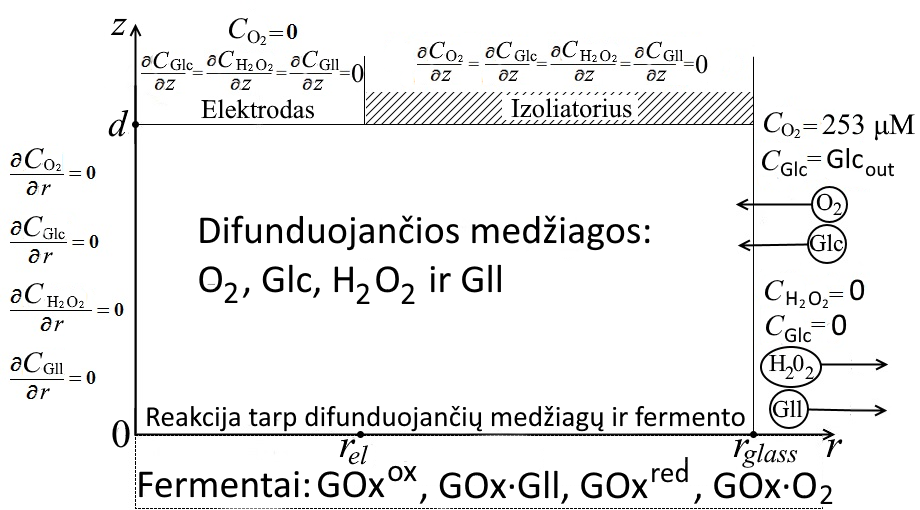
\includegraphics[width=0.8\linewidth]{summary/Model_domainLT.png}
\caption{Modeliavimo srities schema. Pavaizduotos $8$ modeliuotos medžiagos - $4$ difunduojantys reagentai bei $4$ fermento GOx formos, kraštinės sąlygos 4-ioms difunduojančioms medžiagoms ir išorinis srautas.}
\label{fig:santr_Domain}
\end{figure}

Difuzijos procesai išreiškiami antruoju Fiko dėsniu:
\begin{equation}
  \begin{aligned}\label{eq:santr_eq1}
  \frac{\partial C_{O_2}}{\partial t} &= D_{O_2}\,\Delta C_{O_2},\\
  \frac{\partial C_{Glc}}{\partial t} &= D_{Glc}\,\Delta C_{Glc},\\
  \frac{\partial C_{H_2 O_2}}{\partial t} &= D_{H_2 O_2} \,\Delta C_{H_2 O_2},\\
  \frac{\partial C_{Gll}}{\partial t} &= D_{Gll}\,\Delta C_{Gll},  \quad 0<t\leq T,\; 0<z<d,\; 0<r<r_{glass}.
  \end{aligned}
\end{equation}
Šiose lygtyse:
\begin{itemize}
  \item[] $C_{O_2}$, $C_{Glc}$, $C_{H_2 O_2}$ ir $C_{Gll}$ yra atitinkamų difunduojančių re\-a\-gen\-tų koncentracijos, kurios išreiškiamos kaip laiko $t$, er\-dvi\-nių ko\-or\-di\-na\-čių $z$ ir $r$ funkcijos. 
  \item[] $D_{O_2}$, $D_{Glc}$, $D_{H_2 O_2}$ ir $D_{Gll}$ yra difuzijos koeficientai.
  \item[] $d$ yra atstumas tarp fermentu modifikuoto paviršiaus ir elektrodo. Skaitinio eksperimento metu $d$ keičiamas nuo $\SI{1}{\um}$ iki $\SI{120}{\um}$. Tai atitinka elektrodo stumdymą aukštyn ir žemyn cheminio eksperimento metu.
  \item[] $r_{glass} = \SI{80}{\um}$ yra izoliuotos srities spindulys.
  \item[] $T$ yra skaičiavimo eksperimento trukmė, matuojama sekundėmis.
  \item[] Laplaso operatorius $\Delta$ cilindrinėse koordinatėse su centrine simetrija yra
  \begin{equation*}
  \Delta C = \frac{1}{r}\frac{\partial C }{\partial r} \left( r\frac{\partial C }{\partial r} \right) + \frac{\partial^{2} C}{\partial z^{2}}.
  \end{equation*}
\end{itemize}


\chapter*{General conclusions / Bendrosios išvados }
\label{cha:concl_lt}
\addcontentsline{toc}{chapter}{\MakeUppercase{General conclusions / Bendrosios išvados}} 

It is recommended that these conclusions relate directly to the objectives and defending statements of the thesis. 
The conclusions should accurately reflect the results obtained in the dissertation work.
The recommended number of conclusions is 3-5.

\textbf{Note}. Please do a direct translation of the conclusion to Lithuanian language and put them to the \verb|chapter_concl_lt.tex|.


\textbf{In Lithuanian} Šiame skyriuje pateikite sąrašą pagrindinių disertacijos išvadų. Rekomenduojama, kad šios išvados tiesiogiai sietųsi su darbo uždaviniais ir ginamaisiais teiginiais. Išvadose turėtų tiksliai atsispindėti rezultatai gauti disertacijos darbe. 
Rekomenduojamas išvadų kiekis 3-5.

\textbf{Pataba}.Jeigu disertaciją rašote lietuviškai, tuomet išvadas išverskite į anglų kalbą ir pateikite \verb|chapter_concl.tex| faile, kuris būtų naudojamas angliškoje disertacijos santraukoje.
Jeigu disertaciją rašote angliškai, tuomet išverskite į lietuvių kalbą ir pateikite \verb|chapter_concl_lt.tex| faile.

\english  %griztame prie anglu kalbos